\documentclass[]{article}
\usepackage{lmodern}
\usepackage{amssymb,amsmath}
\usepackage{ifxetex,ifluatex}
\usepackage{fixltx2e} % provides \textsubscript
\ifnum 0\ifxetex 1\fi\ifluatex 1\fi=0 % if pdftex
  \usepackage[T1]{fontenc}
  \usepackage[utf8]{inputenc}
\else % if luatex or xelatex
  \ifxetex
    \usepackage{mathspec}
  \else
    \usepackage{fontspec}
  \fi
  \defaultfontfeatures{Ligatures=TeX,Scale=MatchLowercase}
\fi
% use upquote if available, for straight quotes in verbatim environments
\IfFileExists{upquote.sty}{\usepackage{upquote}}{}
% use microtype if available
\IfFileExists{microtype.sty}{%
\usepackage{microtype}
\UseMicrotypeSet[protrusion]{basicmath} % disable protrusion for tt fonts
}{}
\usepackage[margin=1in]{geometry}
\usepackage{hyperref}
\hypersetup{unicode=true,
            pdftitle={flgaCBC},
            pdfauthor={Burnett, JL},
            pdfborder={0 0 0},
            breaklinks=true}
\urlstyle{same}  % don't use monospace font for urls
\usepackage{graphicx,grffile}
\makeatletter
\def\maxwidth{\ifdim\Gin@nat@width>\linewidth\linewidth\else\Gin@nat@width\fi}
\def\maxheight{\ifdim\Gin@nat@height>\textheight\textheight\else\Gin@nat@height\fi}
\makeatother
% Scale images if necessary, so that they will not overflow the page
% margins by default, and it is still possible to overwrite the defaults
% using explicit options in \includegraphics[width, height, ...]{}
\setkeys{Gin}{width=\maxwidth,height=\maxheight,keepaspectratio}
\IfFileExists{parskip.sty}{%
\usepackage{parskip}
}{% else
\setlength{\parindent}{0pt}
\setlength{\parskip}{6pt plus 2pt minus 1pt}
}
\setlength{\emergencystretch}{3em}  % prevent overfull lines
\providecommand{\tightlist}{%
  \setlength{\itemsep}{0pt}\setlength{\parskip}{0pt}}
\setcounter{secnumdepth}{0}
% Redefines (sub)paragraphs to behave more like sections
\ifx\paragraph\undefined\else
\let\oldparagraph\paragraph
\renewcommand{\paragraph}[1]{\oldparagraph{#1}\mbox{}}
\fi
\ifx\subparagraph\undefined\else
\let\oldsubparagraph\subparagraph
\renewcommand{\subparagraph}[1]{\oldsubparagraph{#1}\mbox{}}
\fi

%%% Use protect on footnotes to avoid problems with footnotes in titles
\let\rmarkdownfootnote\footnote%
\def\footnote{\protect\rmarkdownfootnote}

%%% Change title format to be more compact
\usepackage{titling}

% Create subtitle command for use in maketitle
\newcommand{\subtitle}[1]{
  \posttitle{
    \begin{center}\large#1\end{center}
    }
}

\setlength{\droptitle}{-2em}

  \title{flgaCBC}
    \pretitle{\vspace{\droptitle}\centering\huge}
  \posttitle{\par}
    \author{Burnett, JL}
    \preauthor{\centering\large\emph}
  \postauthor{\par}
      \predate{\centering\large\emph}
  \postdate{\par}
    \date{February 20, 2019}

\usepackage{booktabs}
\usepackage{longtable}
\usepackage{array}
\usepackage{multirow}
\usepackage{wrapfig}
\usepackage{float}
\usepackage{colortbl}
\usepackage{pdflscape}
\usepackage{tabu}
\usepackage{threeparttable}
\usepackage{threeparttablex}
\usepackage[normalem]{ulem}
\usepackage{makecell}
\usepackage{xcolor}

\begin{document}
\maketitle

\section{Introduction}\label{introduction}

CBC and BBS have become powerful tools for understanding large-scale
patterns of population changes in North American birds, having been
applied to guilds, and individual species.\\
Restrictions and major biases, however, do apply to these citizen
science data (Dunn et al. 2005). How well do trends in local CBCs mirror
larger trends? Can we use insights from long-term local participants to
identify possible causes of some of these trends? What have local
birders observed that might help explain declines and increases. Habitat
loss, succession, climate, dog fennel, prairie regrowth, drought, cyclic
changes of drying, Are there processes other than actual population
changes creating apparent population changes (superior birding skills
(Sauer et al. 1994; Dunn et al. 2005), more knowledge of where birds
might be hiding? More competition among groups? More bird feeder
watchers (Dunn et al. 2005)? Better techniques such as playbacks of
mobbing or screech owls? Stable populations but decreases caused by an
increasing count effort that can only count a fixed number of
individuals? Declining birding skills as we get older?) Changes in
effort over time (Butcher and McCulloch 1990)

\subsection{On the CBC data}\label{on-the-cbc-data}

\begin{verbatim}
## Warning: Removed 3 rows containing missing values (geom_path).
\end{verbatim}

\begin{figure}
\centering
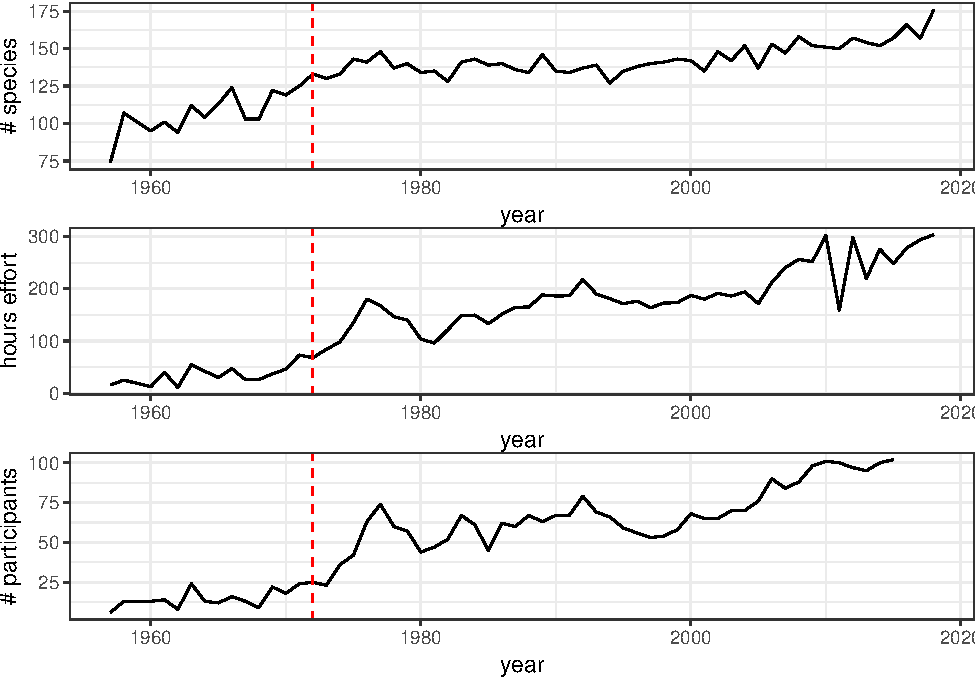
\includegraphics{runThrough_files/figure-latex/effortPlots-1.pdf}
\caption{Annual effort and species richness for the FLGA CBC circle.
Dashed line indicates year we begin analyses.}
\end{figure}

The count format (broken up into 11 teams and all day counts) was
instituted in 1972, so i think that would be a good time to begin.
Therefore, we analze data from 1972 to 2018.

\subsection{Group the species}\label{group-the-species}

In some portions, we present results in groups of species according to
various hypotheses. Species groupings are as follows: Declining, Ag
vics, Endemic, DDT vics, Feeder, Non-native, Urban adapters, North
Florida winter center, Neotropical migrants, Short distance migrants,
Sweetwater (see Table @ref(sppGroupTab)).

\begingroup\fontsize{9}{11}\selectfont

\begin{longtable}{>{\bfseries}l>{\bfseries}ll}
\caption{\label{tab:sppGroupTab}Species groups for analysis}\\
\toprule
sppGroup & family & species\\
\midrule
 & Columbidae & Common Ground-Dove\\

 & Icteridae & Eastern Meadowlark\\

 & Laniidae & Loggerhead Shrike\\

 & Mimidae & Brown Thrasher\\

 & Odontophoridae & Northern Bobwhite\\

 &  & Field Sparrow\\

 &  & Grasshopper Sparrow\\

 & \multirow{-3}{*}{\raggedright\arraybackslash Passerellidae} & Henslow's Sparrow\\

 &  & Northern Flicker\\

\multirow{-10}{*}{\raggedright\arraybackslash Declining} & \multirow{-2}{*}{\raggedright\arraybackslash Picidae} & Red-Headed Woodpecker\\
\cmidrule{1-3}
 &  & Northern Harrier\\

 & \multirow{-2}{*}{\raggedright\arraybackslash Accipitridae} & Red-Tailed Hawk\\

 & Charadriidae & Killdeer\\

 &  & Common Ground-Dove\\

 & \multirow{-2}{*}{\raggedright\arraybackslash Columbidae} & Mourning Dove\\

 & Falconidae & American Kestrel\\

 &  & Boat-Tailed Grackle\\

 &  & Common Grackle\\

 &  & Eastern Meadowlark\\

 & \multirow{-4}{*}{\raggedright\arraybackslash Icteridae} & Red-Winged Blackbird\\

 & Laniidae & Loggerhead Shrike\\

 &  & Brown Thrasher\\

 & \multirow{-2}{*}{\raggedright\arraybackslash Mimidae} & Northern Mockingbird\\

 & Motacillidae & American Pipit\\

 &  & Field Sparrow\\

 &  & Savannah Sparrow\\

 & \multirow{-3}{*}{\raggedright\arraybackslash Passerellidae} & Vesper Sparrow\\

 & Passeridae & House Sparrow\\

 & Turdidae & Eastern Bluebird\\

 & Tyrannidae & Eastern Phoebe\\

\multirow{-21}{*}{\raggedright\arraybackslash Ag vics} & Tytonidae & Barn Owl\\
\cmidrule{1-3}
 & Passerellidae & Bachman's Sparrow\\

 & Picidae & Red-Cockaded Woodpecker\\

\multirow{-3}{*}{\raggedright\arraybackslash Endemic} & Sittidae & Brown-Headed Nuthatch\\
\cmidrule{1-3}
 &  & Bald Eagle\\

 &  & Cooper's Hawk\\

 &  & Red-Shouldered Hawk\\

 & \multirow{-4}{*}{\raggedright\arraybackslash Accipitridae} & Sharp-Shinned Hawk\\

 &  & Merlin\\

 & \multirow{-2}{*}{\raggedright\arraybackslash Falconidae} & Peregrine Falcon\\

 & Pandionidae & Osprey\\

\multirow{-8}{*}{\raggedright\arraybackslash DDT vics} & Phalacrocoracidae & Double-Crested Cormorant\\
\cmidrule{1-3}
 &  & Cooper's Hawk\\

 & \multirow{-2}{*}{\raggedright\arraybackslash Accipitridae} & Sharp-Shinned Hawk\\

 &  & Indigo Bunting\\

 &  & Northern Cardinal\\

 & \multirow{-3}{*}{\raggedright\arraybackslash Cardinalidae} & Painted Bunting\\

 & Columbidae & Mourning Dove\\

 &  & American Crow\\

 & \multirow{-2}{*}{\raggedright\arraybackslash Corvidae} & Blue Jay\\

 &  & American Goldfinch\\

 &  & House Finch\\

 & \multirow{-3}{*}{\raggedright\arraybackslash Fringillidae} & Pine Siskin\\

 &  & Baltimore Oriole\\

 & \multirow{-2}{*}{\raggedright\arraybackslash Icteridae} & Brown-Headed Cowbird\\

 & Laridae & Ring-Billed Gull\\

 &  & Carolina Chickadee\\

 & \multirow{-2}{*}{\raggedright\arraybackslash Paridae} & Tufted Titmouse\\

 & Parulidae & Yellow-Throated Warbler\\

 & Passerellidae & Chipping Sparrow\\

 & Passeridae & House Sparrow\\

 & Picidae & Red-Bellied Woodpecker\\

 & Sittidae & Red-Breasted Nuthatch\\

\multirow{-22}{*}{\raggedright\arraybackslash Feeder} & Troglodytidae & Carolina Wren\\
\cmidrule{1-3}
 &  & Black-Bellied Whistling-Duck\\

 &  & Egyptian Goose\\

 & \multirow{-3}{*}{\raggedright\arraybackslash Anatidae} & Mallard\\

 &  & Eurasian Collared-Dove\\

 &  & Mourning Dove\\

 & \multirow{-3}{*}{\raggedright\arraybackslash Columbidae} & Rock Dove\\

 & Passeridae & House Sparrow\\

\multirow{-8}{*}{\raggedright\arraybackslash Non-native} & Sturnidae & European Starling\\
\cmidrule{1-3}
 & Accipitridae & Red-Shouldered Hawk\\

 &  & Black-Bellied Whistling-Duck\\

 &  & Egyptian Goose\\

 &  & Mallard\\

 &  & Canada Goose\\

 &  & Hooded Merganser\\

 & \multirow{-6}{*}{\raggedright\arraybackslash Anatidae} & Wood Duck\\

 & Cardinalidae & Northern Cardinal\\

 &  & Black Vulture\\

 & \multirow{-2}{*}{\raggedright\arraybackslash Cathartidae} & Turkey Vulture\\

 &  & Eurasian Collared-Dove\\

 &  & Mourning Dove\\

 & \multirow{-3}{*}{\raggedright\arraybackslash Columbidae} & Rock Dove\\

 &  & American Crow\\

 &  & Blue Jay\\

 & \multirow{-3}{*}{\raggedright\arraybackslash Corvidae} & Fish Crow\\

 & Fringillidae & House Finch\\

 &  & Boat-Tailed Grackle\\

 &  & Brown-Headed Cowbird\\

 & \multirow{-3}{*}{\raggedright\arraybackslash Icteridae} & Common Grackle\\

 & Laridae & Ring-Billed Gull\\

 &  & Brown Thrasher\\

 & \multirow{-2}{*}{\raggedright\arraybackslash Mimidae} & Northern Mockingbird\\

 &  & Carolina Chickadee\\

 & \multirow{-2}{*}{\raggedright\arraybackslash Paridae} & Tufted Titmouse\\

 & Passeridae & House Sparrow\\

 & Picidae & Pileated Woodpecker\\

 & Rallidae & Common Gallinule\\

 &  & Eastern Screech-Owl\\

 & \multirow{-2}{*}{\raggedright\arraybackslash Strigidae} & Great Horned Owl\\

 & Sturnidae & European Starling\\

 & Threskiornithidae & White Ibis\\

 &  & Carolina Wren\\

 & \multirow{-2}{*}{\raggedright\arraybackslash Troglodytidae} & House Wren\\

\multirow{-35}{*}{\raggedright\arraybackslash Urban adapters} & Tytonidae & Barn Owl\\
\cmidrule{1-3}
 & Alcedinidae & Belted Kingfisher\\

 & Cardinalidae & Northern Cardinal\\

 & Charadriidae & Killdeer\\

 & Columbidae & Mourning Dove\\

 &  & American Crow\\

 &  & Blue Jay\\

 & \multirow{-3}{*}{\raggedright\arraybackslash Corvidae} & Fish Crow\\

 & Fringillidae & American Goldfinch\\

 & Icteridae & Brown-Headed Cowbird\\

 &  & Brown Thrasher\\

 &  & Gray Catbird\\

 & \multirow{-3}{*}{\raggedright\arraybackslash Mimidae} & Northern Mockingbird\\

 &  & Carolina Chickadee\\

 & \multirow{-2}{*}{\raggedright\arraybackslash Paridae} & Tufted Titmouse\\

 &  & Black-And-White Warbler\\

 &  & Common Yellowthroat\\

 &  & Orange-Crowned Warbler\\

 &  & Palm Warbler\\

 &  & Pine Warbler\\

 &  & Yellow-Rumped Warbler\\

 & \multirow{-7}{*}{\raggedright\arraybackslash Parulidae} & Yellow-Throated Warbler\\

 &  & Chipping Sparrow\\

 & \multirow{-2}{*}{\raggedright\arraybackslash Passerellidae} & Swamp Sparrow\\

 &  & Downy Woodpecker\\

 &  & Red-Bellied Woodpecker\\

 & \multirow{-3}{*}{\raggedright\arraybackslash Picidae} & Yellow-Bellied Sapsucker\\

 & Polioptilidae & Blue-Gray Gnatcatcher\\

 & Regulidae & Ruby-Crowned Kinglet\\

 & Scolopacidae & Wilson's Snipe\\

 &  & Carolina Wren\\

 &  & House Wren\\

 & \multirow{-3}{*}{\raggedright\arraybackslash Troglodytidae} & Sedge Wren\\

 &  & American Robin\\

 & \multirow{-2}{*}{\raggedright\arraybackslash Turdidae} & Eastern Bluebird\\

 & Tyrannidae & Eastern Phoebe\\

 &  & Blue-Headed Vireo\\

\multirow{-37}{*}{\raggedright\arraybackslash North Florida winter center} & \multirow{-2}{*}{\raggedright\arraybackslash Vireonidae} & White-Eyed Vireo\\
\cmidrule{1-3}
 & Apodidae & Vaux's Swift\\

 & Caprimulgidae & Eastern Whip-Poor-Will\\

 &  & Dickcissel\\

 &  & Indigo Bunting\\

 &  & Painted Bunting\\

 &  & Rose-Breasted Grosbeak\\

 &  & Summer Tanager\\

 & \multirow{-6}{*}{\raggedright\arraybackslash Cardinalidae} & Western Tanager\\

 &  & Baltimore Oriole\\

 &  & Bullock's Oriole\\

 & \multirow{-3}{*}{\raggedright\arraybackslash Icteridae} & Orchard Oriole\\

 & Icteriidae & Yellow-Breasted Chat\\

 &  & American Redstart\\

 &  & Black-And-White Warbler\\

 &  & Black-Throated Blue Warbler\\

 &  & Black-Throated Green Warbler\\

 &  & Blackburnian Warbler\\

 &  & Blue-Winged Warbler\\

 &  & Louisiana Waterthrush\\

 &  & Magnolia Warbler\\

 &  & Nashville Warbler\\

 &  & Northern Parula\\

 &  & Northern Waterthrush\\

 &  & Ovenbird\\

 &  & Prairie Warbler\\

 &  & Tennessee Warbler\\

 &  & Yellow Warbler\\

 & \multirow{-16}{*}{\raggedright\arraybackslash Parulidae} & Wilson's Warbler\\

 &  & Black-Chinned Hummingbird\\

 &  & Ruby-Throated Hummingbird\\

 & \multirow{-3}{*}{\raggedright\arraybackslash Trochilidae} & Rufous Hummingbird\\

 & Turdidae & Wood Thrush\\

 &  & Ash-Throated Flycatcher\\

 &  & Brown-Crested Flycatcher\\

 &  & Eastern Kingbird\\

 &  & Least Flycatcher\\

 &  & Western Kingbird\\

 & \multirow{-6}{*}{\raggedright\arraybackslash Tyrannidae} & Vermilion Flycatcher\\

\multirow{-39}{*}{\raggedright\arraybackslash Neotropical migrants} & Vireonidae & Yellow-Throated Vireo\\
\cmidrule{1-3}
 &  & Northern Harrier\\

 & \multirow{-2}{*}{\raggedright\arraybackslash Accipitridae} & Sharp-Shinned Hawk\\

 & Certhiidae & Brown Creeper\\

 &  & Pine Siskin\\

 & \multirow{-2}{*}{\raggedright\arraybackslash Fringillidae} & Purple Finch\\

 & Gruidae & Sandhill Crane\\

 &  & Common Grackle\\

 &  & Red-Winged Blackbird\\

 & \multirow{-3}{*}{\raggedright\arraybackslash Icteridae} & Rusty Blackbird\\

 &  & Dark-Eyed Junco\\

 &  & Eastern Towhee\\

 &  & Fox Sparrow\\

 &  & Song Sparrow\\

 &  & Vesper Sparrow\\

 &  & White-Throated Sparrow\\

 & \multirow{-7}{*}{\raggedright\arraybackslash Passerellidae} & White-Crowned Sparrow\\

 & Regulidae & Golden-Crowned Kinglet\\

 & Scolopacidae & American Woodcock\\

 & Sittidae & Red-Breasted Nuthatch\\

 & Troglodytidae & Winter Wren\\

\multirow{-21}{*}{\raggedright\arraybackslash Short distance migrants} & Turdidae & Hermit Thrush\\
\cmidrule{1-3}
 & Accipitridae & Snail Kite\\

 & Anatidae & Blue-Winged Teal\\

 & Anhingidae & Anhinga\\

 & Aramidae & Limpkin\\

 &  & American Bittern\\

 &  & Least Bittern\\

 &  & Great Blue Heron\\

 &  & Little Blue Heron\\

 &  & Tricolored Heron\\

 &  & Green Heron\\

 &  & Black-Crowned Night-Heron\\

 & \multirow{-8}{*}{\raggedright\arraybackslash Ardeidae} & Yellow-Crowned Night-Heron\\

 & Ciconiidae & Wood Stork\\

 & Phalacrocoracidae & Double-Crested Cormorant\\

 &  & King Rail\\

 &  & Purple Gallinule\\

 &  & Sora\\

 & \multirow{-4}{*}{\raggedright\arraybackslash Rallidae} & Virginia Rail\\

 &  & White Ibis\\

 &  & Glossy Ibis\\

 & \multirow{-3}{*}{\raggedright\arraybackslash Threskiornithidae} & White-Faced Ibis\\

\multirow{-22}{*}{\raggedright\arraybackslash Sweetwater} & Troglodytidae & Marsh Wren\\
\bottomrule
\end{longtable}

\endgroup{}

\section{Statistical analysis of population
trends}\label{statistical-analysis-of-population-trends}

\subsection{Model structure}\label{model-structure}

We estimated species population trends in the Gainesville, Florida
Christmas Bird Count (CBC; National Audubon Society REF) circle (FLGA)
for the period of 1972 to 2015 using generalized additive models (GAMs,
Hastie and Tibshirani 1990; Wood 2006). GAMs are a flexible
implementation of generalized linear models in cases where species'
populations exhibit non-linear trends. GAMs optimize the predictability
of the relationship between the response and predictor variable(s) while
accounting for the noise associated with year-to-year fluctuations in
species counts.

We ran two types of analyses: (i) species-level trends and (ii)
group-level trends.

\subsubsection{Species-level trends}\label{species-level-trends}

This model includes a factor for species identity. A smooth is produced
for each species over time, and is also included as a fixed effect:

\begin{equation} 
g(E(y_i)) = \beta_0 f(year_i_species) + species + \epsilon_i, \\
y_i ~ some exp. distribution
\end{equation}

\subsubsection{Group trends}\label{group-trends}

@ref(tab:sppGroupTab)). Next, we analyzed individual species trends. We
analyzed individual species' trends using the a generalized additive
model:

\begin{itemize}
\item
  Most species trends were non-linear over the study period. GAM
  optimizes the residuals by fitting knots in the model (count, response
  value), so if the trend is linear, it will fit it.
\item
  ARound 1980 the hours effort and number of participants increased
  linearally, therefore we did not fit a smooth to the hours effort (see
  @ref(fig:effortPlots)).
\item
  We controlled for temporal autocorrelation by taking first, second,
  adn third differences (AR1, AR2, and AR3). We chose the best fitting
  model for each species by running likelihood ratios
\item
  A GAM basically a GLM where the linear preditor(s) are influenced by
  some unknown smooth function, and a GAMM is a GLMM where ``\ldots{}''
\item
  ``for a Poisson model the expected value after log transformation is
  modelled to be linearly dependent on the explanatory variables''"
\item
\end{itemize}

\subsection{Analysis results}\label{analysis-results}

\begingroup\fontsize{9}{11}\selectfont

\begin{longtable}{l}
\caption{\label{tab:sppAnalysedTab}Species analysed.}\\
\toprule
x\\
\midrule
Wood Duck\\
Mallard\\
Blue-Winged Teal\\
Hooded Merganser\\
Northern Bobwhite\\
\addlinespace
Double-Crested Cormorant\\
Anhinga\\
Great Blue Heron\\
Little Blue Heron\\
Tricolored Heron\\
\addlinespace
Green Heron\\
Black-Crowned Night-Heron\\
White Ibis\\
Glossy Ibis\\
Black Vulture\\
\addlinespace
Turkey Vulture\\
Osprey\\
Northern Harrier\\
Sharp-Shinned Hawk\\
Cooper's Hawk\\
\addlinespace
Bald Eagle\\
Red-Shouldered Hawk\\
Red-Tailed Hawk\\
King Rail\\
Virginia Rail\\
\addlinespace
Sora\\
Sandhill Crane\\
Killdeer\\
Wilson's Snipe\\
American Woodcock\\
\addlinespace
Ring-Billed Gull\\
Rock Dove\\
Mourning Dove\\
Eastern Screech-Owl\\
Great Horned Owl\\
\addlinespace
Belted Kingfisher\\
Red-Headed Woodpecker\\
Red-Bellied Woodpecker\\
Yellow-Bellied Sapsucker\\
Downy Woodpecker\\
\addlinespace
Northern Flicker\\
Pileated Woodpecker\\
American Kestrel\\
Eastern Phoebe\\
Loggerhead Shrike\\
\addlinespace
White-Eyed Vireo\\
Blue-Headed Vireo\\
Blue Jay\\
American Crow\\
Fish Crow\\
\addlinespace
Carolina Chickadee\\
Tufted Titmouse\\
Brown-Headed Nuthatch\\
House Wren\\
Sedge Wren\\
\addlinespace
Marsh Wren\\
Carolina Wren\\
Blue-Gray Gnatcatcher\\
Ruby-Crowned Kinglet\\
Eastern Bluebird\\
\addlinespace
Hermit Thrush\\
American Robin\\
Gray Catbird\\
Northern Mockingbird\\
Brown Thrasher\\
\addlinespace
European Starling\\
American Pipit\\
Ovenbird\\
Black-And-White Warbler\\
Orange-Crowned Warbler\\
\addlinespace
Common Yellowthroat\\
Palm Warbler\\
Pine Warbler\\
Yellow-Rumped Warbler\\
Yellow-Throated Warbler\\
\addlinespace
Eastern Towhee\\
Chipping Sparrow\\
Field Sparrow\\
Vesper Sparrow\\
Savannah Sparrow\\
\addlinespace
Song Sparrow\\
Swamp Sparrow\\
White-Throated Sparrow\\
Northern Cardinal\\
Red-Winged Blackbird\\
\addlinespace
Eastern Meadowlark\\
Common Grackle\\
Boat-Tailed Grackle\\
Brown-Headed Cowbird\\
Baltimore Oriole\\
\addlinespace
American Goldfinch\\
House Sparrow\\
\bottomrule
\end{longtable}

\endgroup{}

\section{References not yet defined in
.bib}\label{references-not-yet-defined-in-.bib}

Fewster, Rachel M., et al. ``Analysis of population trends for farmland
birds using generalized additive models.'' Ecology 81.7 (2000):
1970-1984. Hastie, Trevor J., and Robert J. Tibshirani. Generalized
additive models. Vol. 43. CRC Press, 1990. R Core Team (2015). R: A
language and environment for statistical computing. R Founding for
Statistical Computing, Vienna, Austria. URL
\url{https://www.R-project.org/}. Wood, S.N. (2006) Generalized Additive
Models: An Introduction with R. Chapman and Hall/CRC.


\end{document}
